\documentclass[11pt,letterpaper]{article}

% --- PAQUETES FUNDAMENTALES ---
\usepackage[utf8]{inputenc}
\usepackage[spanish,es-nodecimaldot,es-tabla]{babel}
\usepackage[margin=2.2cm,top=2.5cm,bottom=2.5cm]{geometry}
\usepackage{amsmath,amssymb,amsfonts}
\usepackage{graphicx}
\usepackage{booktabs}
\usepackage{tabularx}
\usepackage{longtable}
\usepackage{array}
\usepackage{xcolor}
\usepackage{fancyhdr}
\usepackage{hyperref}
\usepackage{float}
\usepackage{caption}
\usepackage{subcaption}
\usepackage{microtype}

% --- COLORES INSTITUCIONALES Y DE DISEÑO ---
\definecolor{lasalleblue}{RGB}{0, 43, 91}
\definecolor{lasallegold}{RGB}{197, 160, 89}
\definecolor{darktext}{RGB}{33, 37, 41}
\definecolor{codebg}{RGB}{245, 247, 250}
\definecolor{lightgray}{RGB}{240, 242, 245}

% --- CONFIGURACIÓN DE HIPERVÍNCULOS ---
\hypersetup{
    colorlinks=true,
    linkcolor=lasalleblue,
    citecolor=lasalleblue,
    urlcolor=lasalleblue,
    pdftitle={Fase 1: Planteamiento del Problema, Descripción y EDA},
    pdfauthor={Yerson León Montañez}
}

% --- ENCABEZADOS Y PIES DE PÁGINA ---
\pagestyle{fancy}
\fancyhf{}
\fancyhead[L]{\small \textcolor{lasalleblue}{\textbf{Universidad de La Salle}} | Maestría en IA}
\fancyhead[R]{\small \textcolor{darktext}{Fase 1: Planteamiento y EDA}}
\fancyfoot[L]{\small \textcolor{darktext}{Ciencia de Datos — Docente: Fabián Camilo Castro Riveros}}
\fancyfoot[R]{\small \textcolor{darktext}{Página \thepage}}
\renewcommand{\headrulewidth}{0.8pt}
\renewcommand{\footrulewidth}{0.4pt}

% --- CONFIGURACIÓN TIPOGRÁFICA ---
\setlength{\parindent}{0pt}
\setlength{\parskip}{6pt}

\begin{document}

% --- PORTADA INSTITUCIONAL ---
\begin{titlepage}
    \centering
    \vspace*{0.5cm}
    {\huge \textbf{\textcolor{lasalleblue}{UNIVERSIDAD DE LA SALLE}}}\\[0.3cm]
    {\large \textbf{Facultad de Ingeniería — Departamento de Ciencias Básicas}}\\[0.2cm]
    {\large \textbf{Maestría en Inteligencia Artificial}}\\[1.8cm]

    \rule{\linewidth}{1.5pt}\\[0.4cm]
    {\LARGE \textbf{\textcolor{lasalleblue}{PROYECTO INTEGRADOR DE CIENCIA DE DATOS E INTELIGENCIA ARTIFICIAL}}}\\[0.3cm]
    {\Large \textbf{Fase 1: Planteamiento del Problema, Descripción Técnica y Análisis Exploratorio de Datos (EDA)}}\\[0.2cm]
    {\normalsize \textbf{Entregable Técnico 1 (Ponderación: 20\%)}}\\[0.4cm]
    \rule{\linewidth}{1.5pt}\\[2.0cm]

    \begin{minipage}[t]{0.48\textwidth}
        \textbf{Estudiante:}\\
        Yerson León Montañez\\
        \texttt{yeleon36@unisalle.edu.co}\\
        Código Estudiantil: Maestría en IA
    \end{minipage}
    \hfill
    \begin{minipage}[t]{0.48\textwidth}
        \begin{flushright}
            \textbf{Docente Titular:}\\
            Fabián Camilo Castro Riveros\\
            \textit{Cátedra de Ciencia de Datos}\\
            Periodo Académico: 2026-II
        \end{flushright}
    \end{minipage}

    \vfill
    {\large Bogotá D.C., Colombia\\ \textbf{28 de octubre de 2026}}
\end{titlepage}

\newpage
\tableofcontents
\newpage

% ==============================================================================
% SECCIÓN 1: FORMULACIÓN DEL PROBLEMA Y OBJETIVOS
% ==============================================================================
\section{Formulación del Problema y Objetivos del Proyecto}

\subsection{Contextualización del Dominio e Impacto de la Solución Analítica}
En la industria global de telecomunicaciones, la retención de suscriptores constituye uno de los desafíos operacionales y financieros más críticos. La pérdida no planificada de clientes (\textit{Customer Churn}) impacta directamente en el flujo de caja recurrente (\textit{Monthly Recurring Revenue} - MRR) e incrementa el costo marginal por cliente atendido. Múltiples investigaciones empíricas demuestran que captar un suscriptor nuevo representa un costo entre cinco y veinticinco veces superior a retener un cliente fidelizado, considerando los gastos de adquisición comercial, subsidios de infraestructura y comisiones.

Asimismo, la deserción en telecomunicaciones es un fenómeno multifactorial inducido por presiones tarifarias, calidad de conectividad, soporte posventa deficiente y la oferta de servicios suplementarios (tales como seguridad cibernética, copias de seguridad y asistencia técnica). El desarrollo de una solución basada en el ciclo completo de Ciencia de Datos y Aprendizaje Automático permite transformar registros operacionales pasivos en capacidades predictivas y prescriptivas. Al predecir con alta precisión el abandono, estimar la facturación monetaria acumulada (\textit{Customer Lifetime Value} - LTV) y segmentar la base instalada mediante agrupamiento no supervisado, la empresa puede focalizar incentivos de retención, optimizar costos operativos y personalizar paquetes de servicio en tiempo real.

\subsection{Preguntas de Investigación}

\subsubsection{Pregunta Principal}
\begin{quote}
    \textbf{¿Cuáles son los patrones de comportamiento de consumo, características de suscripción contractual y perfiles tecnológicos que determinan de manera estadísticamente significativa la probabilidad de deserción (\textit{Churn}) de un cliente de telecomunicaciones, y cómo pueden estructurarse en modelos predictivos y de segmentación para optimizar la retención y anticipar el valor facturado acumulado?}
\end{quote}

\subsubsection{Preguntas Secundarias}
\begin{enumerate}
    \item \textbf{Pregunta Secundaria 1 (Estructura Contractual y Financiera):} ¿En qué medida la modalidad de contrato (mensual vs. anual/bianual) y el método de facturación (electrónica con débito automático vs. cheque electrónico) condicionan la tasa de deserción del usuario?
    \item \textbf{Pregunta Secundaria 2 (Servicios de Valor Agregado):} ¿Constituye la suscripción a servicios complementarios de protección y soporte (\textit{TechSupport}, \textit{OnlineSecurity}, \textit{OnlineBackup}) una barrera de salida efectiva que reduce el riesgo de fuga frente a clientes con servicios puramente de conectividad?
    \item \textbf{Pregunta Secundaria 3 (Modelación Continua y Relación No Lineal):} ¿Cuál es el grado de interdependencia cuantitativa entre la antigüedad del cliente (\textit{tenure}), los cargos mensuales facturados (\textit{MonthlyCharges}) y los cobros históricos acumulados (\textit{TotalCharges}), y cómo puede modelarse matemáticamente para detectar anomalías y anticipar el LTV del cliente?
\end{enumerate}

\subsection{Objetivos del Proyecto en Formato SMART}

\subsubsection{Objetivo General}
\begin{quote}
    \textbf{Desarrollar y validar un sistema analítico predictivo y prescriptivo de Ciencia de Datos para la industria de telecomunicaciones, integrando modelos de regresión regularizada para la estimación de ingresos acumulados, algoritmos supervisados de clasificación y un Perceptrón Multicapa (MLP) en PyTorch para la predicción de la deserción, complementados con segmentación no supervisada (K-Means y Jerárquico/DBSCAN) y un dashboard interactivo desplegado en la web, en el lapso académico del 20 de octubre al 28 de noviembre de 2026.}
\end{quote}

\subsubsection{Objetivos Específicos}
\begin{enumerate}
    \item \textbf{Objetivo Específico 1 — EDA, Diagnóstico de Calidad y Ficha Técnica [Fase 1]:}\\
    \textbf{S} (Específico): Caracterizar estadísticamente las 21 variables del dataset de telecomunicaciones mediante métricas univariadas (momentos de forma, tendencia y dispersión), matrices de correlación bivariada, pruebas de independencia de Chi-cuadrado ($\chi^2$) y auditoría de datos faltantes y atípicos.\\
    \textbf{M} (Medible): Procesar el 100\% de las 7,043 observaciones, cuantificar la significancia estadística ($p$-valor $< 0.05$) y el tamaño del efecto ($V$ de Cramér) para el total de variables cualitativas.\\
    \textbf{A} (Alcanzable): Ejecutado mediante librerías científicas (\texttt{pandas}, \texttt{scipy.stats}, \texttt{seaborn}) y documentado en formato LaTeX y Jupyter Notebook reproducible.\\
    \textbf{R} (Relevante): Establece la base empírica indispensable para el tratamiento de valores nulos encubiertos y la prevención de fuga de información (\textit{data leakage}).\\
    \textbf{T} (Temporal): Completado y entregado al 01 de noviembre de 2026.

    \item \textbf{Objetivo Específico 2 — Preprocesamiento, Ingeniería de Variables y Modelos de Aprendizaje [Fases 2 y 3]:}\\
    \textbf{S} (Específico): Implementar una tubería de preprocesamiento rigurosa (imputación justificada, codificación One-Hot sin data leakage, escalado ajustado sobre entrenamiento) y entrenar modelos de regresión lineal regularizada (Ridge/Lasso), ensambles de árboles (Random Forest, XGBoost), clasificadores diversos y una red neuronal MLP en PyTorch.\\
    \textbf{M} (Medible): Superar un coeficiente de determinación $R^2 \ge 0.80$ en la estimación de cargos y alcanzar un $F_1\text{-score} \ge 0.78$ junto con un $AUC\text{-}ROC \ge 0.84$ en la clase minoritaria de deserción.\\
    \textbf{A} (Alcanzable): Respaldado en validación cruzada estratificada (\textit{Stratified K-Fold}) y balanceo algorítmico.\\
    \textbf{R} (Relevante): Garantiza solidez metodológica y capacidad de generalización sobre datos no observados.\\
    \textbf{T} (Temporal): Implementado y optimizado entre el 03 de noviembre y el 22 de noviembre de 2026.

    \item \textbf{Objetivo Específico 3 — Puesta en Producción, Interpretabilidad y Visualización Interactiva [Fase 4]:}\\
    \textbf{S} (Específico): Desplegar una aplicación web interactiva en Streamlit que integre tarjetas ejecutivas de KPI, un simulador de inferencia en tiempo real para predicción de Churn y visualización del espacio de agrupamiento de clientes asistido por análisis de componentes principales (PCA), complementado con interpretabilidad global y local mediante valores SHAP.\\
    \textbf{M} (Medible): Tiempos de respuesta de inferencia menores a 500 ms y 100\% de disponibilidad del dashboard web.\\
    \textbf{A} (Alcanzable): Implementado a través de librerías nativas de Python y estructuración modular del repositorio.\\
    \textbf{R} (Relevante): Facilita la toma de decisiones basada en datos por parte de directores comerciales y de fidelización.\\
    \textbf{T} (Temporal): Finalizado y sustentado oralmente el 28 de noviembre de 2026.
\end{enumerate}

% ==============================================================================
% SECCIÓN 2: FICHA TÉCNICA DEL DATASET
% ==============================================================================
\section{Ficha Técnica del Dataset y Diccionario de Datos}

\subsection{Ficha Técnica Institucional}
El conjunto de datos seleccionado cumple con la totalidad de los criterios restrictivos establecidos en la Sección 2 de la Guía Técnica del Proyecto Integrador: proviene de un repositorio público reconocido, no constituye un conjunto didáctico básico restringido (como Iris o Titanic), supera con holgura los 600 registros limpios (7,043 observaciones), cuenta con 21 variables mixtas (cualitativas y cuantitativas) y permite formular simultáneamente problemas de regresión, clasificación y agrupamiento.

\begin{table}[H]
    \centering
    \small
    \caption{Ficha técnica del conjunto de datos.}
    \label{tab:ficha_tecnica}
    \begin{tabularx}{\linewidth}{p{4.2cm}X}
        \toprule
        \textbf{Descriptor Metodológico} & \textbf{Detalle Técnico} \\
        \midrule
        \textbf{Nombre del Dataset} & \textit{Telco Customer Churn (IBM Business Analytics Dataset)} \\
        \textbf{Repositorio de Origen} & Kaggle Datasets / IBM Community Analytics \\
        \textbf{URL Oficial de Acceso} & \url{https://www.kaggle.com/datasets/blastchar/telco-customer-churn} \\
        \textbf{Tipo de Licencia} & Creative Commons Zero (CC0: Public Domain) / Apache License 2.0 \\
        \textbf{Fecha de Extracción} & 28 de octubre de 2026 \\
        \textbf{Formato de Almacenamiento} & Comma-Separated Values (\texttt{.csv}), codificación UTF-8 \\
        \textbf{Volumen del Conjunto} & 7,043 registros (filas) y 21 atributos (columnas) \\
        \textbf{Uso en Regresión} & Estimación de \texttt{TotalCharges} o \texttt{MonthlyCharges} (Variables cuantitativas continuas) \\
        \textbf{Uso en Clasificación} & Predicción del estado de deserción \texttt{Churn} (Variable categórica binaria: Sí / No) \\
        \textbf{Uso en Clustering} & Segmentación no supervisada por \texttt{tenure}, consumo tarifario y tenencia de servicios \\
        \bottomrule
    \end{tabularx}
\end{table}

\subsection{Diccionario Exhaustivo de Variables}
A continuación se detalla la semántica de cada uno de los 21 campos del conjunto de datos, especificando su tipología estadística formal, rol analítico en el proyecto y rango de valores permitidos.

\begin{table}[H]
    \centering
    \scriptsize
    \caption{Diccionario de datos completo y tipificación estadística.}
    \label{tab:diccionario_datos}
    \begin{tabularx}{\linewidth}{p{2.8cm}p{3.2cm}Xp{2.6cm}}
        \toprule
        \textbf{Nombre Columna} & \textbf{Tipo Estadístico} & \textbf{Descripción Funcional en el Dominio} & \textbf{Valores Permitidos / Rango} \\
        \midrule
        \texttt{customerID} & Cualitativa Nominal & Identificador alfanumérico único por suscriptor & Formato alfanumérico (\texttt{XXXX-XXXXX}) \\
        \texttt{gender} & Cualitativa Nominal (Binaria) & Género biológico reportado por el cliente & \texttt{Female}, \texttt{Male} \\
        \texttt{SeniorCitizen} & Cualitativa Nominal (Binaria) & Indicador si el cliente es adulto mayor ($\ge 65$ años) & \texttt{0} (No), \texttt{1} (Sí) \\
        \texttt{Partner} & Cualitativa Nominal (Binaria) & Si el suscriptor convive con cónyuge o pareja & \texttt{Yes}, \texttt{No} \\
        \texttt{Dependents} & Cualitativa Nominal (Binaria) & Si el cliente tiene personas dependientes económicamente & \texttt{Yes}, \texttt{No} \\
        \texttt{tenure} & Cuantitativa Discreta & Cantidad de meses de permanencia en la empresa & Enteros en $[0, 72]$ \\
        \texttt{PhoneService} & Cualitativa Nominal (Binaria) & Suscripción al servicio de telefonía fija & \texttt{Yes}, \texttt{No} \\
        \texttt{MultipleLines} & Cualitativa Nominal & Tenencia de múltiples líneas telefónicas & \texttt{No phone service}, \texttt{No}, \texttt{Yes} \\
        \texttt{InternetService} & Cualitativa Nominal & Proveedor de conexión a internet contratada & \texttt{DSL}, \texttt{Fiber optic}, \texttt{No} \\
        \texttt{OnlineSecurity} & Cualitativa Nominal & Servicio de seguridad perimetral antivirus/malware & \texttt{No internet service}, \texttt{No}, \texttt{Yes} \\
        \texttt{OnlineBackup} & Cualitativa Nominal & Almacenamiento seguro en la nube & \texttt{No internet service}, \texttt{No}, \texttt{Yes} \\
        \texttt{DeviceProtection}& Cualitativa Nominal & Póliza de protección y reemplazo de hardware & \texttt{No internet service}, \texttt{No}, \texttt{Yes} \\
        \texttt{TechSupport} & Cualitativa Nominal & Soporte técnico prioritario especializado & \texttt{No internet service}, \texttt{No}, \texttt{Yes} \\
        \texttt{StreamingTV} & Cualitativa Nominal & Transmisión de televisión en línea vía internet & \texttt{No internet service}, \texttt{No}, \texttt{Yes} \\
        \texttt{StreamingMovies}& Cualitativa Nominal & Transmisión de películas y series vía internet & \texttt{No internet service}, \texttt{No}, \texttt{Yes} \\
        \texttt{Contract} & Cualitativa Ordinal & Duración y modalidad legal del contrato & \texttt{Month-to-month}, \texttt{One year}, \texttt{Two year} \\
        \texttt{PaperlessBilling}& Cualitativa Nominal (Binaria) & Facturación ecológica digital en lugar de física & \texttt{Yes}, \texttt{No} \\
        \texttt{PaymentMethod} & Cualitativa Nominal & Mecanismo de pago registrado por el usuario & \texttt{Electronic check}, \texttt{Mailed check}, \texttt{Bank transfer}, \texttt{Credit card} \\
        \texttt{MonthlyCharges} & Cuantitativa Continua & Tarifa mensual devengada por el cliente & Real en $[18.25, 118.75]$ USD \\
        \texttt{TotalCharges} & Cuantitativa Continua & Importe monetario total acumulado facturado & Real en $[18.80, 8684.80]$ USD \\
        \texttt{Churn} & Cualitativa Nominal (Binaria) & \textbf{Variable Objetivo:} Abandono en el último mes & \texttt{Yes}, \texttt{No} \\
        \bottomrule
    \end{tabularx}
\end{table}

% ==============================================================================
% SECCIÓN 3: ANÁLISIS EXPLORATORIO DE DATOS (EDA)
% ==============================================================================
\section{Análisis Exploratorio de Datos (EDA) Exhaustivo}

\subsection{Diagnóstico Riguroso de Calidad de Datos}
La auditoría de integridad sobre la estructura tabular cruda evaluó duplicados, consistencia de claves primarias y presencia de nulos aparentes o encubiertos.

\begin{itemize}
    \item \textbf{Duplicidad de Registros:} Se comprobó la unicidad de las filas. La cantidad de registros repetidos globales es $0$ ($0.0\%$), y la clave primaria \texttt{customerID} no presenta ninguna duplicidad (7,043 identificadores unívocos).
    \item \textbf{Valores Faltantes Encubiertos:} De las 21 columnas, 20 presentan un $0.0\%$ estricto de valores faltantes. No obstante, una inspección de tipos reveló que \texttt{TotalCharges} fue leída inicialmente como tipo \texttt{object} (cadena de texto). La inspección profunda detectó exactamente $11$ registros donde el valor registrado correspondía a un espacio en blanco (\texttt{' '}).
    \item \textbf{Diagnóstico del Mecanismo de Falta (MCAR vs. MAR vs. MNAR):}\\
    Al cruzar los 11 registros donde \texttt{TotalCharges} está en blanco con las demás características, se evidenció que en el $100\%$ de los casos ($11/11$), la variable \texttt{tenure} es idénticamente igual a $0$. Corresponden a clientes en su primer ciclo de facturación que aún no han recibido su cobro histórico.\\
    Por tanto, el mecanismo de falta no es \textit{Missing Completely at Random} (MCAR) ni \textit{Missing Not at Random} (MNAR), sino estrictamente \textbf{Missing at Random (MAR)}, pues la probabilidad de ausencia está matemáticamente explicada por otra variable completamente observada (\texttt{tenure = 0}). Esto justifica teóricamente que en la Fase 2 dichos valores no deben descartarse, sino imputarse deterministicamente a cero (\texttt{TotalCharges = 0.0}).
\end{itemize}

\subsection{Detección y Tratamiento Formal de Valores Atípicos (Outliers)}
Para evaluar la existencia de valores atípicos en las tres dimensiones continuas (\texttt{tenure}, \texttt{MonthlyCharges} y \texttt{TotalCharges}), se implementaron dos criterios matemáticos formales:

\begin{enumerate}
    \item \textbf{Criterio del Rango Intercuartílico de Tukey (IQR):}
    \begin{equation}
        IQR = Q_3 - Q_1, \quad L_{inf} = Q_1 - 1.5 \cdot IQR, \quad L_{sup} = Q_3 + 1.5 \cdot IQR
    \end{equation}
    \item \textbf{Criterio de Estandarización de Puntuación $Z$ ($Z$-Score):}
    \begin{equation}
        Z_i = \frac{x_i - \mu}{\sigma}, \quad \text{Atípico si } |Z_i| > 3
    \end{equation}
\end{enumerate}

\begin{table}[H]
    \centering
    \caption{Diagnóstico cuantitativo de valores atípicos mediante criterios IQR y $Z$-score.}
    \label{tab:outliers}
    \resizebox{\linewidth}{!}{
    \begin{tabular}{lrrrrrr}
        \toprule
        \textbf{Variable} & \textbf{$L_{inf}$ (IQR)} & \textbf{$L_{sup}$ (IQR)} & \textbf{Atípicos IQR ($n$)} & \textbf{\% IQR} & \textbf{Atípicos $|Z|>3$ ($n$)} & \textbf{\% $|Z|>3$} \\
        \midrule
        \texttt{tenure} & $-60.00$ & $124.00$ & $0$ & $0.000\%$ & $0$ & $0.000\%$ \\
        \texttt{MonthlyCharges} & $-46.02$ & $171.38$ & $0$ & $0.000\%$ & $0$ & $0.000\%$ \\
        \texttt{TotalCharges} & $-4688.48$ & $8884.67$ & $0$ & $0.000\%$ & $0$ & $0.000\%$ \\
        \bottomrule
    \end{tabular}
    }
\end{table}

\begin{figure}[H]
    \centering
    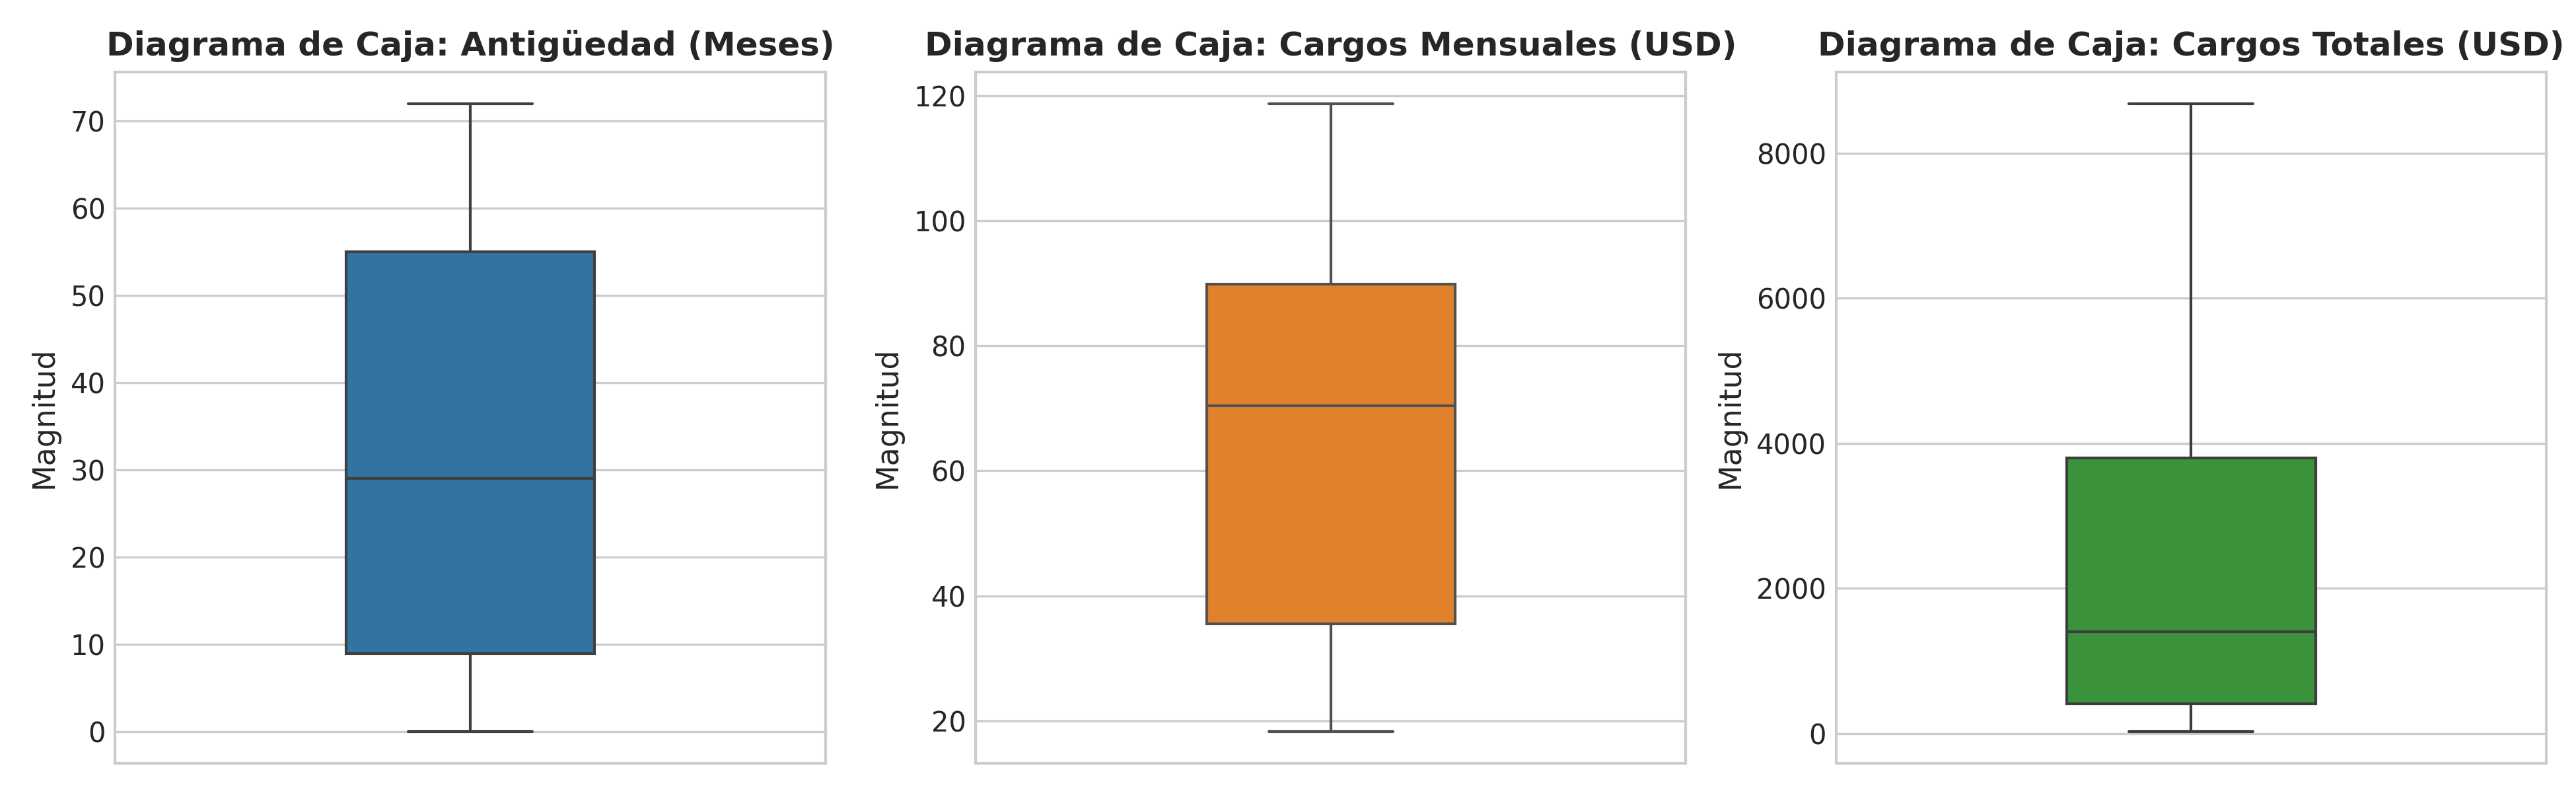
\includegraphics[width=0.95\linewidth]{figures/fig2_outliers_boxplots.png}
    \caption{Diagramas de caja (\textit{boxplots}) para las variables cuantitativas continuas.}
    \label{fig:boxplots}
\end{figure}

\textbf{Interpretación:} Como se aprecia en la Tabla \ref{tab:outliers} y en la Figura \ref{fig:boxplots}, ninguna de las tres variables continuas presenta observaciones fuera de los límites de Tukey ni fuera del intervalo de tres desviaciones estándar. Esto ocurre porque \texttt{tenure} está naturalmente acotada por las políticas de retención ($0$ a $72$ meses), los cobros mensuales corresponden a planes tarifarios estructurados ($\approx \$18$ a $\$118$) y los cobros totales están acotados por el producto de ambas dimensiones.

\subsection{Análisis Univariado Cuantitativo y Momentos de Forma}
Se estimaron los cuatro momentos estadísticos (media, varianza/desviación, asimetría y curtosis) para las variables continuas.

\begin{itemize}
    \item \textbf{Asimetría de Fisher-Pearson ($g_1$):}
    \begin{equation}
        g_1 = \frac{\frac{1}{n} \sum_{i=1}^n (x_i - \bar{x})^3}{\left[\frac{1}{n} \sum_{i=1}^n (x_i - \bar{x})^2\right]^{3/2}}
    \end{equation}
    \item \textbf{Exceso de Curtosis de Fisher ($g_2$):}
    \begin{equation}
        g_2 = \frac{\frac{1}{n} \sum_{i=1}^n (x_i - \bar{x})^4}{\left[\frac{1}{n} \sum_{i=1}^n (x_i - \bar{x})^2\right]^2} - 3
    \end{equation}
\end{itemize}

\begin{table}[H]
    \centering
    \caption{Medidas univariadas de tendencia central, dispersión y momentos de forma.}
    \label{tab:univariado_cuantitativo}
    \resizebox{\linewidth}{!}{
    \begin{tabular}{lrrrrrrrr}
        \toprule
        \textbf{Variable} & \textbf{Media} & \textbf{Mediana} & \textbf{Desv. Est.} & \textbf{IQR} & \textbf{Mínimo} & \textbf{Máximo} & \textbf{Asimetría ($g_1$)} & \textbf{Curtosis ($g_2$)} \\
        \midrule
        \texttt{tenure} & $32.37$ & $29.00$ & $24.56$ & $46.00$ & $0.00$ & $72.00$ & $+0.2395$ & $-1.3874$ \\
        \texttt{MonthlyCharges} & $64.76$ & $70.35$ & $30.09$ & $54.35$ & $18.25$ & $118.75$ & $-0.2205$ & $-1.2573$ \\
        \texttt{TotalCharges} & $2283.30$ & $1397.48$ & $2266.77$ & $3393.29$ & $18.80$ & $8684.80$ & $+0.9616$ & $-0.2318$ \\
        \bottomrule
    \end{tabular}
    }
\end{table}

\begin{figure}[H]
    \centering
    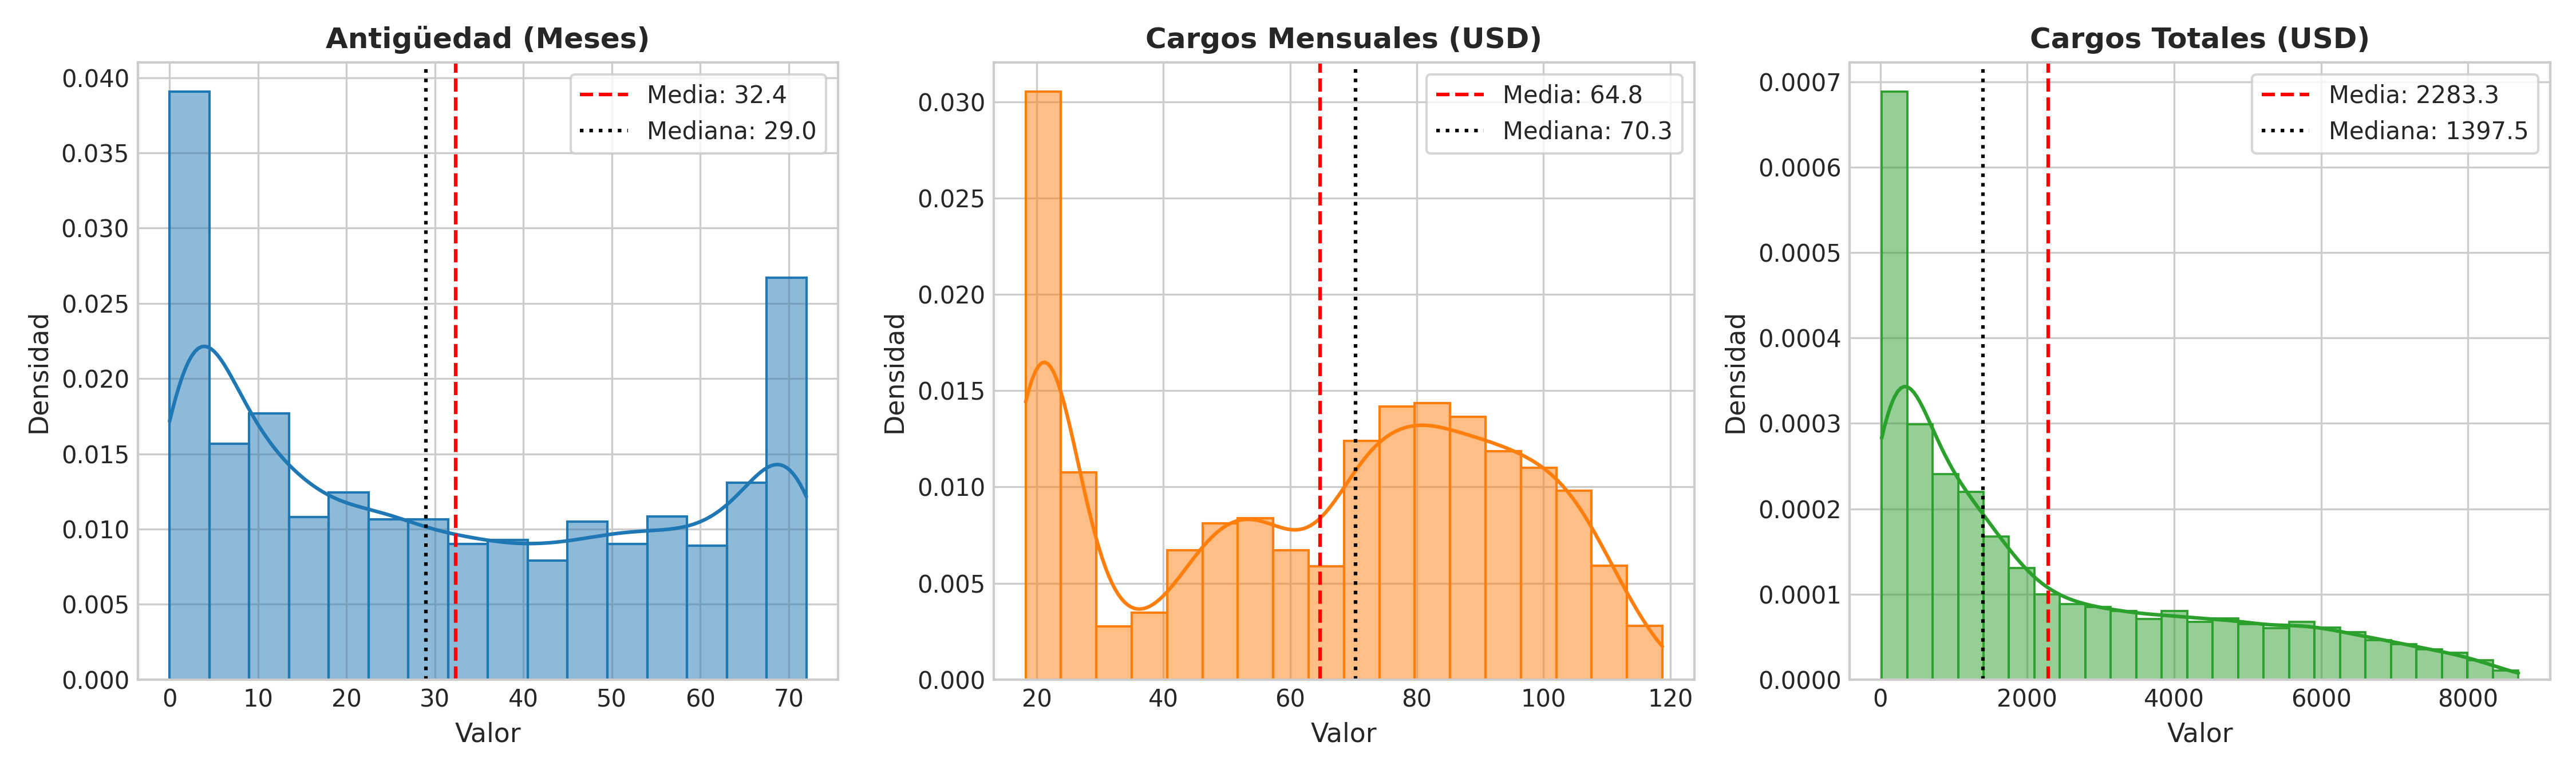
\includegraphics[width=\linewidth]{figures/fig1_univariate_numerical.png}
    \caption{Distribuciones univariadas con estimación de densidad por kernel (KDE), medias y medianas.}
    \label{fig:univariado_kde}
\end{figure}

\textbf{Diagnóstico Estadístico de las Distribuciones:}
\begin{itemize}
    \item \textbf{Antigüedad (\texttt{tenure}):} Presenta una distribución platicúrtica ($g_2 = -1.3874$) fuertemente bimodal (Figura \ref{fig:univariado_kde}). Existen dos concentraciones poblacionales extremas: suscriptores en su primer año ($<12$ meses) y clientes de lealtad extrema ($>60$ meses).
    \item \textbf{Cargos Mensuales (\texttt{MonthlyCharges}):} Muestra igualmente una morfología platicúrtica bimodal ($g_2 = -1.2573$), con un primer pico en planes básicos de solo telefonía ($\approx \$20$) y un segundo pico amplio en usuarios con planes empaquetados de banda ancha y streaming ($\$70 - \$90$).
    \item \textbf{Cargos Totales (\texttt{TotalCharges}):} Evidencia una marcada asimetría positiva a la derecha ($g_1 = +0.9616$), donde la media ($\$2283.30$) supera drásticamente a la mediana ($\$1397.48$). Esto sugiere que en la Fase 2 convendrá ensayar transformaciones logarítmicas o Box-Cox para estabilizar la varianza en los modelos lineales.
\end{itemize}

\subsection{Distribución de Clases de la Variable Objetivo (\texttt{Churn})}
La variable objetivo \texttt{Churn} exhibe $5,174$ registros para la clase negativa (\texttt{No}, $73.46\%$) y $1,869$ registros para la clase positiva (\texttt{Yes}, $26.54\%$). Se identifica un \textbf{desbalance moderado} (proporción aproximada $3:1$). Esto exige implementar en la Fase 2 y Fase 3 técnicas de muestreo estratificado (\textit{Stratified Split}), optimización basada en $F_1\text{-score}$ / $AUC\text{-}ROC$, y ajuste de pesos de clase (\texttt{class\_weight='balanced'}) para evitar sesgos hacia la clase mayoritaria.

\subsection{Análisis Bivariado y Correlación Numérica}
Se estimaron los coeficientes de correlación paramétrica lineal de Pearson ($r$) y no paramétrica monótona de Spearman ($\rho$) entre las variables cuantitativas continuas:

\begin{table}[H]
    \centering
    \small
    \caption{Matrices de correlación de Pearson (triángulo inferior/izquierda) y Spearman (triángulo superior/derecha).}
    \label{tab:correlaciones}
    \begin{tabular}{lrrr}
        \toprule
        \textbf{Métrica / Variable} & \textbf{\texttt{tenure}} & \textbf{\texttt{MonthlyCharges}} & \textbf{\texttt{TotalCharges}} \\
        \midrule
        \textbf{Pearson ($r$):} & & & \\
        \texttt{tenure} & $1.0000$ & $0.2479$ & $0.8259$ \\
        \texttt{MonthlyCharges} & $0.2479$ & $1.0000$ & $0.6511$ \\
        \texttt{TotalCharges} & $0.8259$ & $0.6511$ & $1.0000$ \\
        \midrule
        \textbf{Spearman ($\rho$):} & & & \\
        \texttt{tenure} & $1.0000$ & $0.2764$ & $0.8892$ \\
        \texttt{MonthlyCharges} & $0.2764$ & $1.0000$ & $0.6383$ \\
        \texttt{TotalCharges} & $0.8892$ & $0.6383$ & $1.0000$ \\
        \bottomrule
    \end{tabular}
\end{table}

\begin{figure}[H]
    \centering
    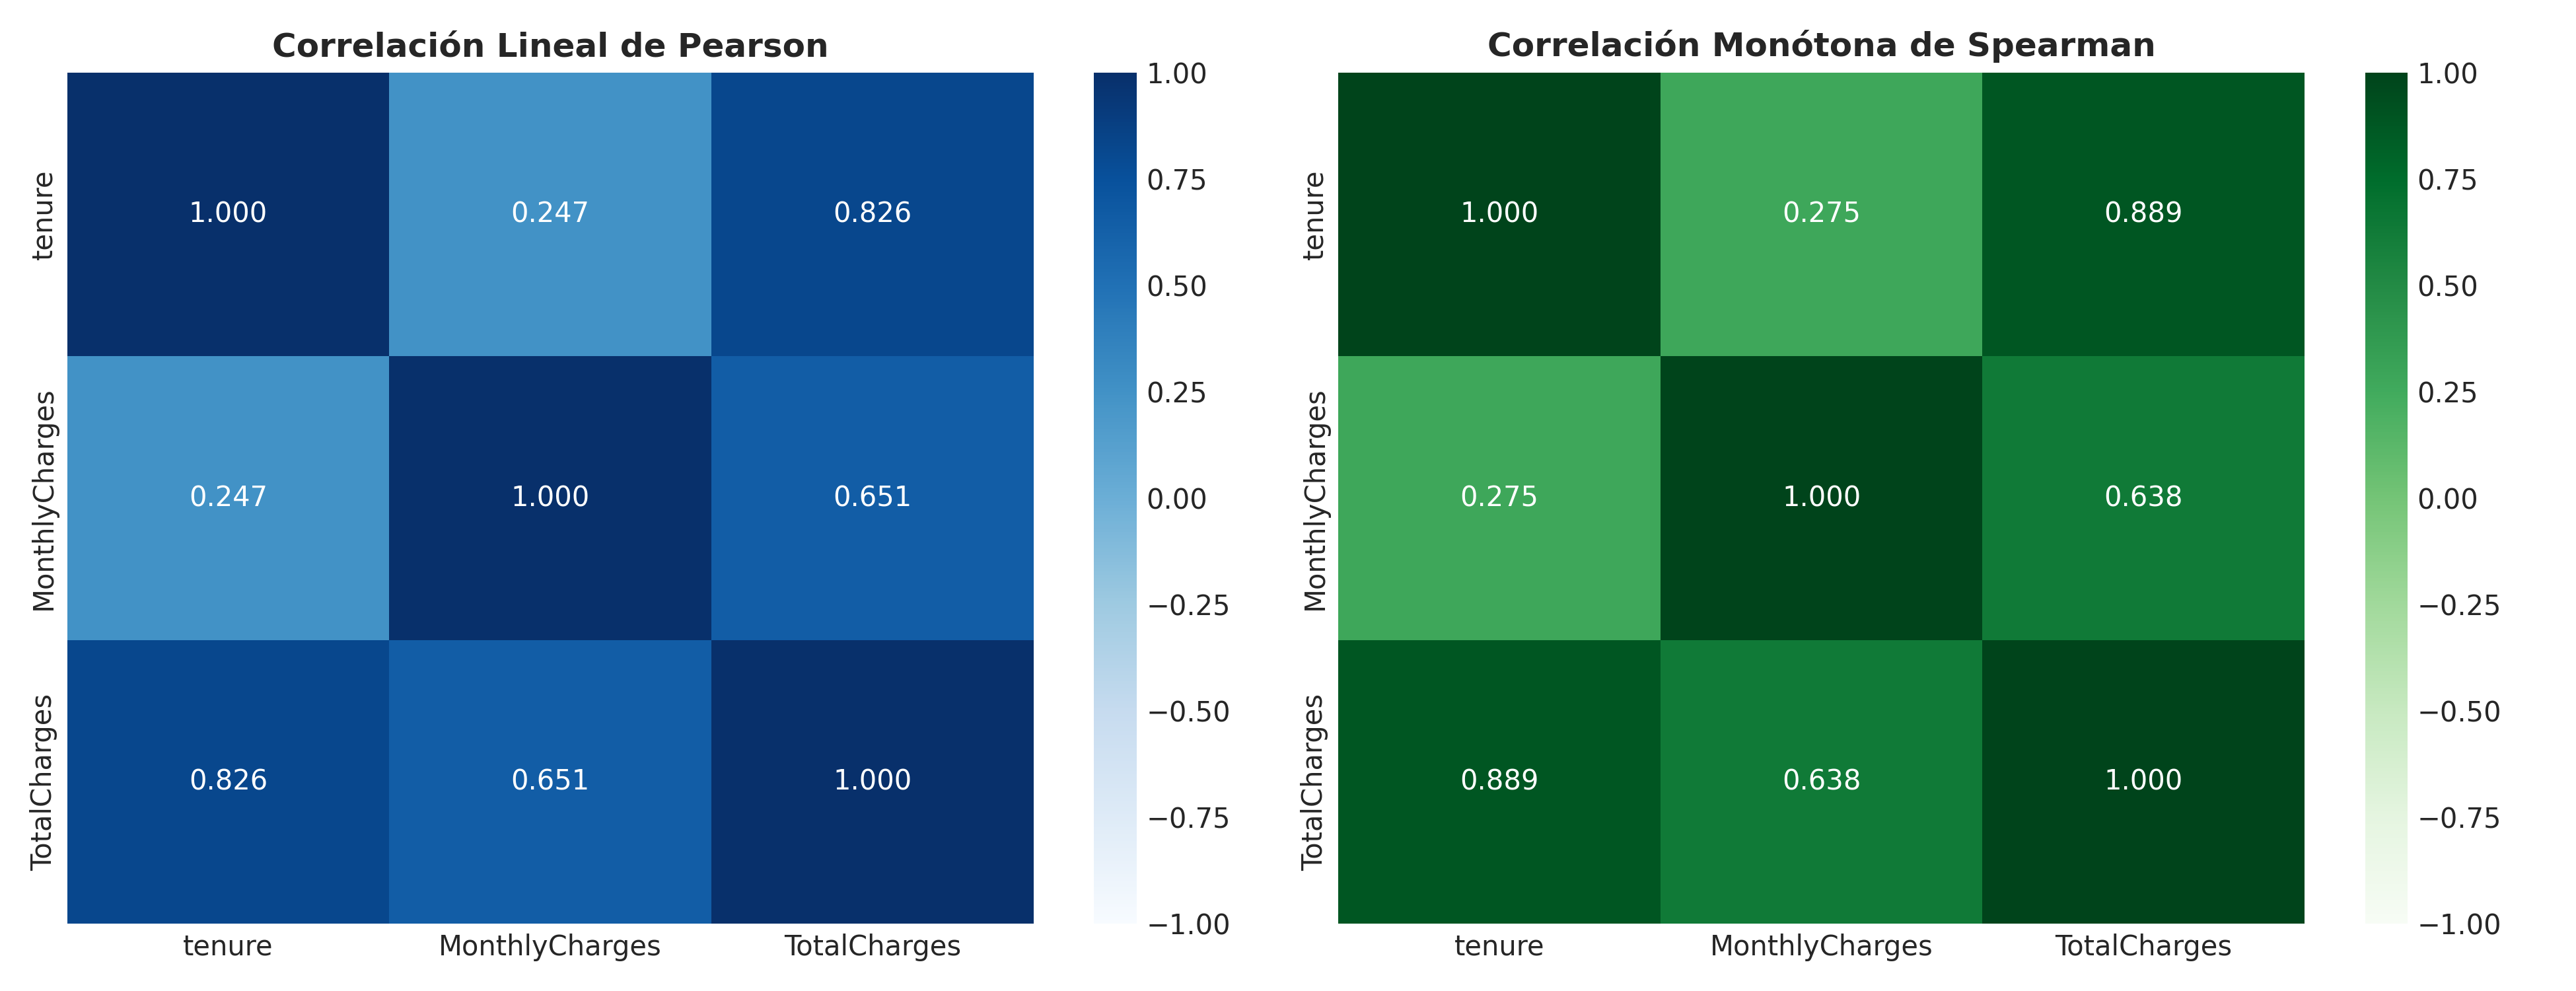
\includegraphics[width=0.92\linewidth]{figures/fig3_correlation_matrices.png}
    \caption{Mapas de calor de las correlaciones numéricas de Pearson y Spearman.}
    \label{fig:heatmaps}
\end{figure}

\begin{figure}[H]
    \centering
    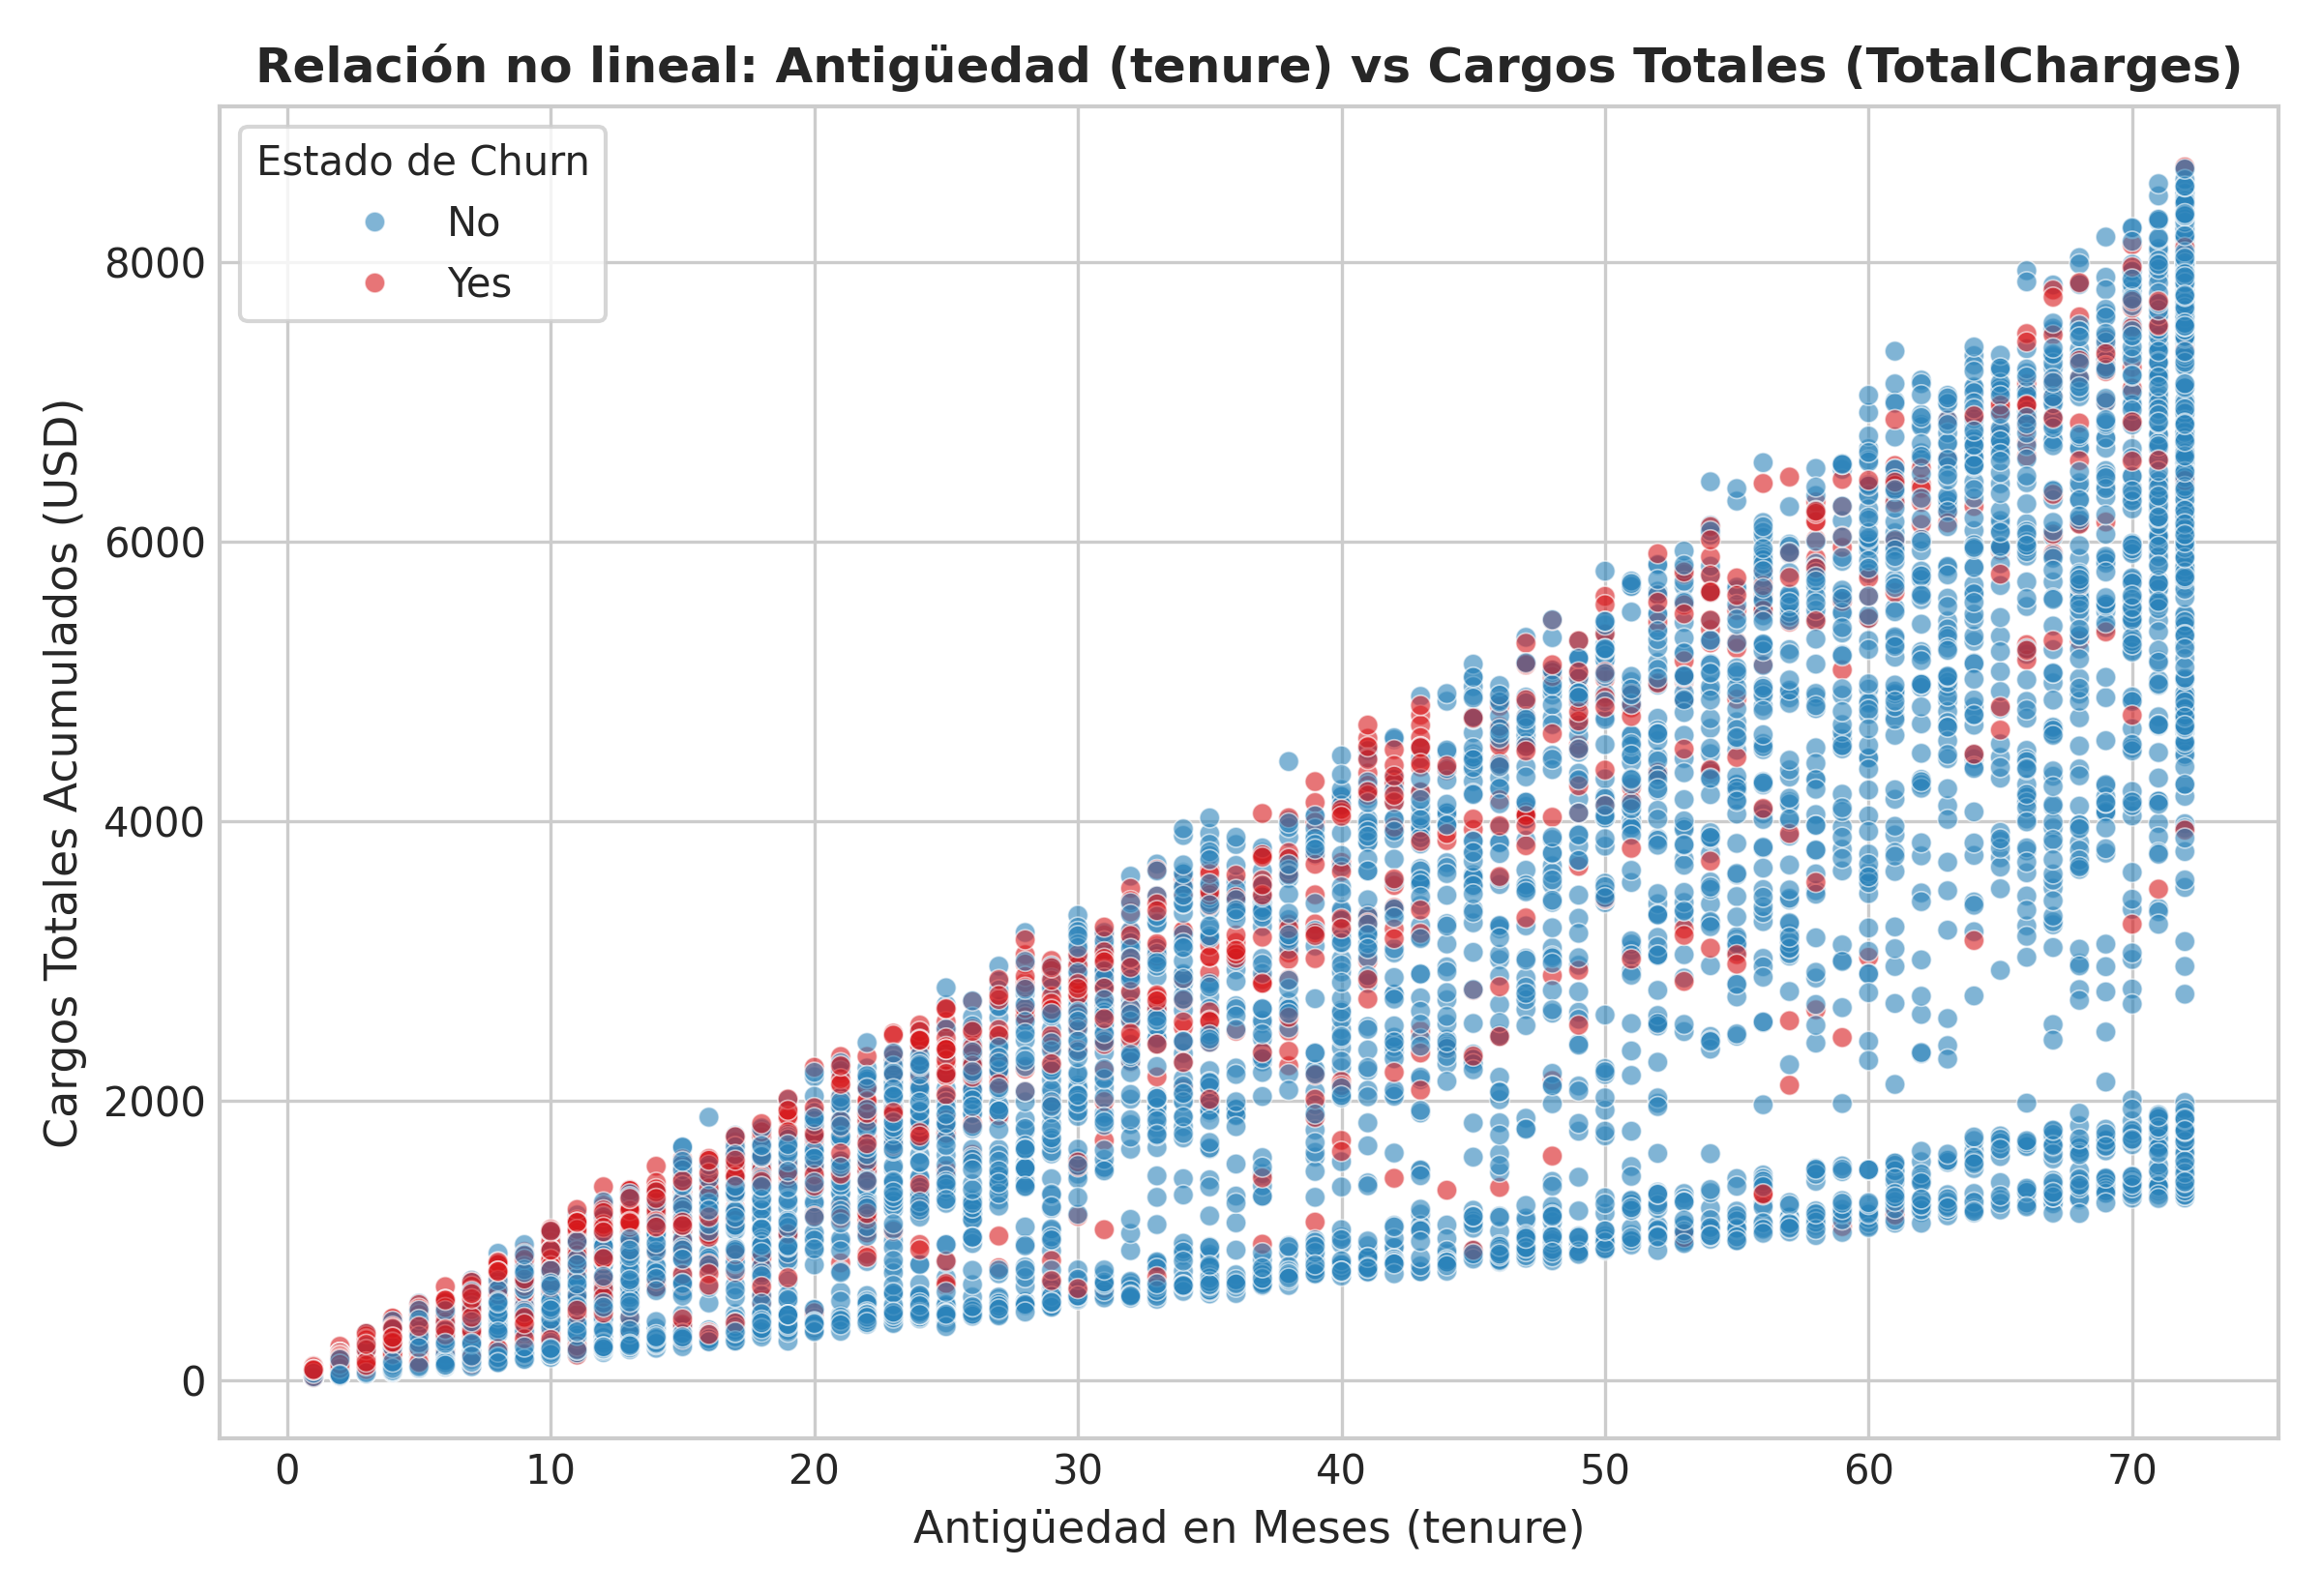
\includegraphics[width=0.75\linewidth]{figures/fig5_bivariate_scatter.png}
    \caption{Diagrama de dispersión bivariado \texttt{tenure} vs. \texttt{TotalCharges} categorizado por deserción.}
    \label{fig:scatter_churn}
\end{figure}

\textbf{Hallazgos Bivariados Clave:}
\begin{enumerate}
    \item Existe una asociación monótona casi perfecta entre la antigüedad y los cargos totales ($\rho = 0.8892$), superando a la correlación lineal de Pearson ($r = 0.8259$). Como ilustra la Figura \ref{fig:scatter_churn}, la dispersión adopta una estructura de embudo con pendientes diferenciadas según la tarifa mensual.
    \item Los clientes desertores (\textit{puntos rojos en la Figura \ref{fig:scatter_churn}}) se concentran masivamente en las franjas de baja antigüedad ($0 - 15$ meses), confirmando que el mayor riesgo de abandono se produce durante el primer año de contrato.
\end{enumerate}

\subsection{Pruebas de Independencia \texorpdfstring{$\chi^2$}{Chi-cuadrado} y Asociación de Variables Cualitativas}
Para evaluar la relación entre cada variable categórica y la variable objetivo \texttt{Churn}, se construyeron tablas de contingencia y se computaron las pruebas de independencia de Chi-cuadrado ($\chi^2$), así como el tamaño del efecto mediante la $V$ de Cramér:

\begin{equation}
    \chi^2 = \sum_{i=1}^r \sum_{j=1}^c \frac{(O_{ij} - E_{ij})^2}{E_{ij}}, \qquad V = \sqrt{\frac{\chi^2}{n \cdot \min(r-1, c-1)}}
\end{equation}

\begin{table}[H]
    \centering
    \caption{Pruebas de independencia de Chi-cuadrado y coeficiente $V$ de Cramér frente a \texttt{Churn}.}
    \label{tab:chi2_results}
    \resizebox{\linewidth}{!}{
    \begin{tabular}{lrrrcp{3.8cm}}
        \toprule
        \textbf{Variable Categórica} & \textbf{Estadístico $\chi^2$} & \textbf{Grados Lib. ($df$)} & \textbf{$p$-valor} & \textbf{$V$ de Cramér} & \textbf{Intensidad Asociación} \\
        \midrule
        \texttt{Contract} & $1184.60$ & $2$ & $5.86 \times 10^{-258}$ & $0.4101$ & \textbf{Fuerte} ($V > 0.30$) \\
        \texttt{OnlineSecurity} & $850.00$ & $2$ & $2.66 \times 10^{-185}$ & $0.3474$ & \textbf{Fuerte} ($V > 0.30$) \\
        \texttt{TechSupport} & $828.20$ & $2$ & $1.44 \times 10^{-180}$ & $0.3429$ & \textbf{Fuerte} ($V > 0.30$) \\
        \texttt{InternetService} & $732.31$ & $2$ & $9.57 \times 10^{-160}$ & $0.3225$ & \textbf{Fuerte} ($V > 0.30$) \\
        \texttt{PaymentMethod} & $648.14$ & $3$ & $3.68 \times 10^{-140}$ & $0.3034$ & \textbf{Fuerte} ($V > 0.30$) \\
        \texttt{OnlineBackup} & $601.81$ & $2$ & $2.08 \times 10^{-131}$ & $0.2923$ & Moderada ($0.15 \le V \le 0.30$) \\
        \texttt{DeviceProtection} & $558.42$ & $2$ & $5.51 \times 10^{-122}$ & $0.2816$ & Moderada ($0.15 \le V \le 0.30$) \\
        \texttt{StreamingMovies} & $375.66$ & $2$ & $2.67 \times 10^{-82}$ & $0.2310$ & Moderada ($0.15 \le V \le 0.30$) \\
        \texttt{StreamingTV} & $374.20$ & $2$ & $5.53 \times 10^{-82}$ & $0.2305$ & Moderada ($0.15 \le V \le 0.30$) \\
        \texttt{PaperlessBilling} & $258.28$ & $1$ & $4.07 \times 10^{-58}$ & $0.1915$ & Moderada ($0.15 \le V \le 0.30$) \\
        \texttt{Dependents} & $189.13$ & $1$ & $4.92 \times 10^{-43}$ & $0.1639$ & Moderada ($0.15 \le V \le 0.30$) \\
        \texttt{SeniorCitizen} & $159.43$ & $1$ & $1.51 \times 10^{-36}$ & $0.1505$ & Moderada ($0.15 \le V \le 0.30$) \\
        \texttt{Partner} & $158.73$ & $1$ & $2.14 \times 10^{-36}$ & $0.1501$ & Moderada ($0.15 \le V \le 0.30$) \\
        \texttt{MultipleLines} & $11.33$ & $2$ & $3.46 \times 10^{-3}$ & $0.0401$ & Débil ($V < 0.15$) \\
        \texttt{PhoneService} & $0.92$ & $1$ & $0.3388$ & $0.0114$ & \textit{No significativo} ($p \ge 0.05$) \\
        \texttt{gender} & $0.48$ & $1$ & $0.4866$ & $0.0083$ & \textit{No significativo} ($p \ge 0.05$) \\
        \bottomrule
    \end{tabular}
    }
\end{table}

\begin{figure}[H]
    \centering
    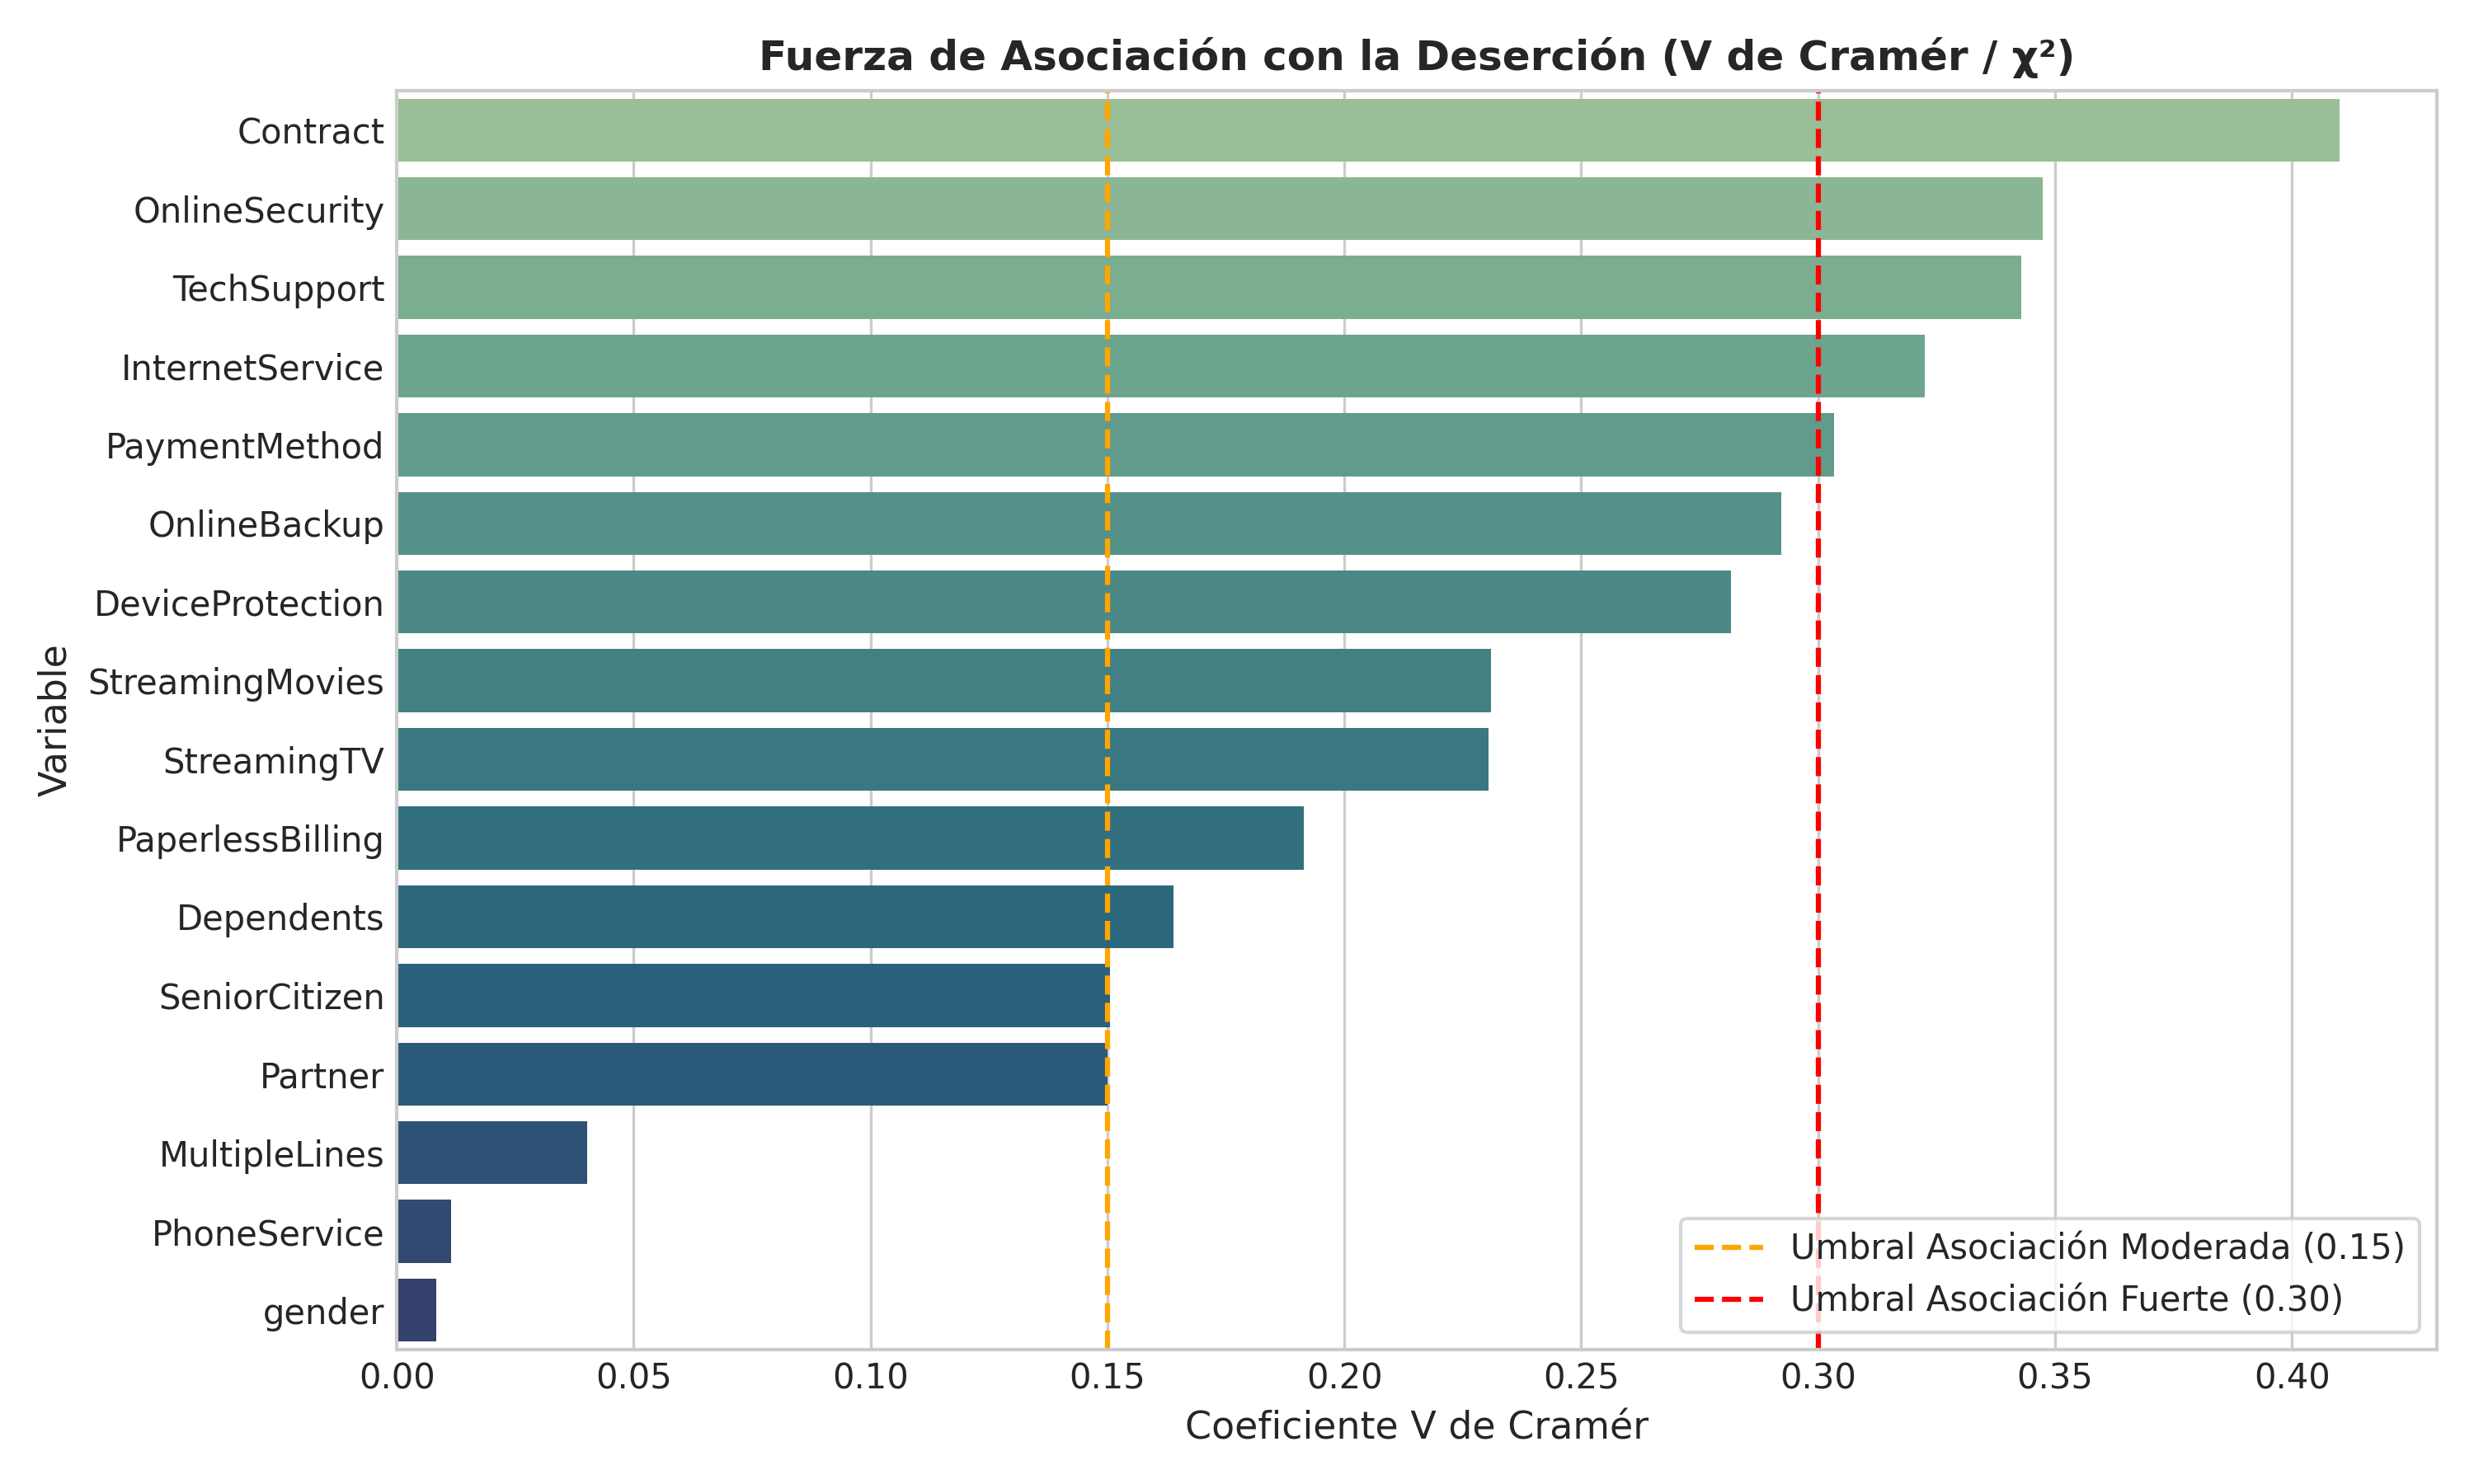
\includegraphics[width=0.88\linewidth]{figures/fig6_cramer_v_association.png}
    \caption{Fuerza de asociación categórica evaluada con el coeficiente $V$ de Cramér.}
    \label{fig:cramer_v}
\end{figure}

\begin{figure}[H]
    \centering
    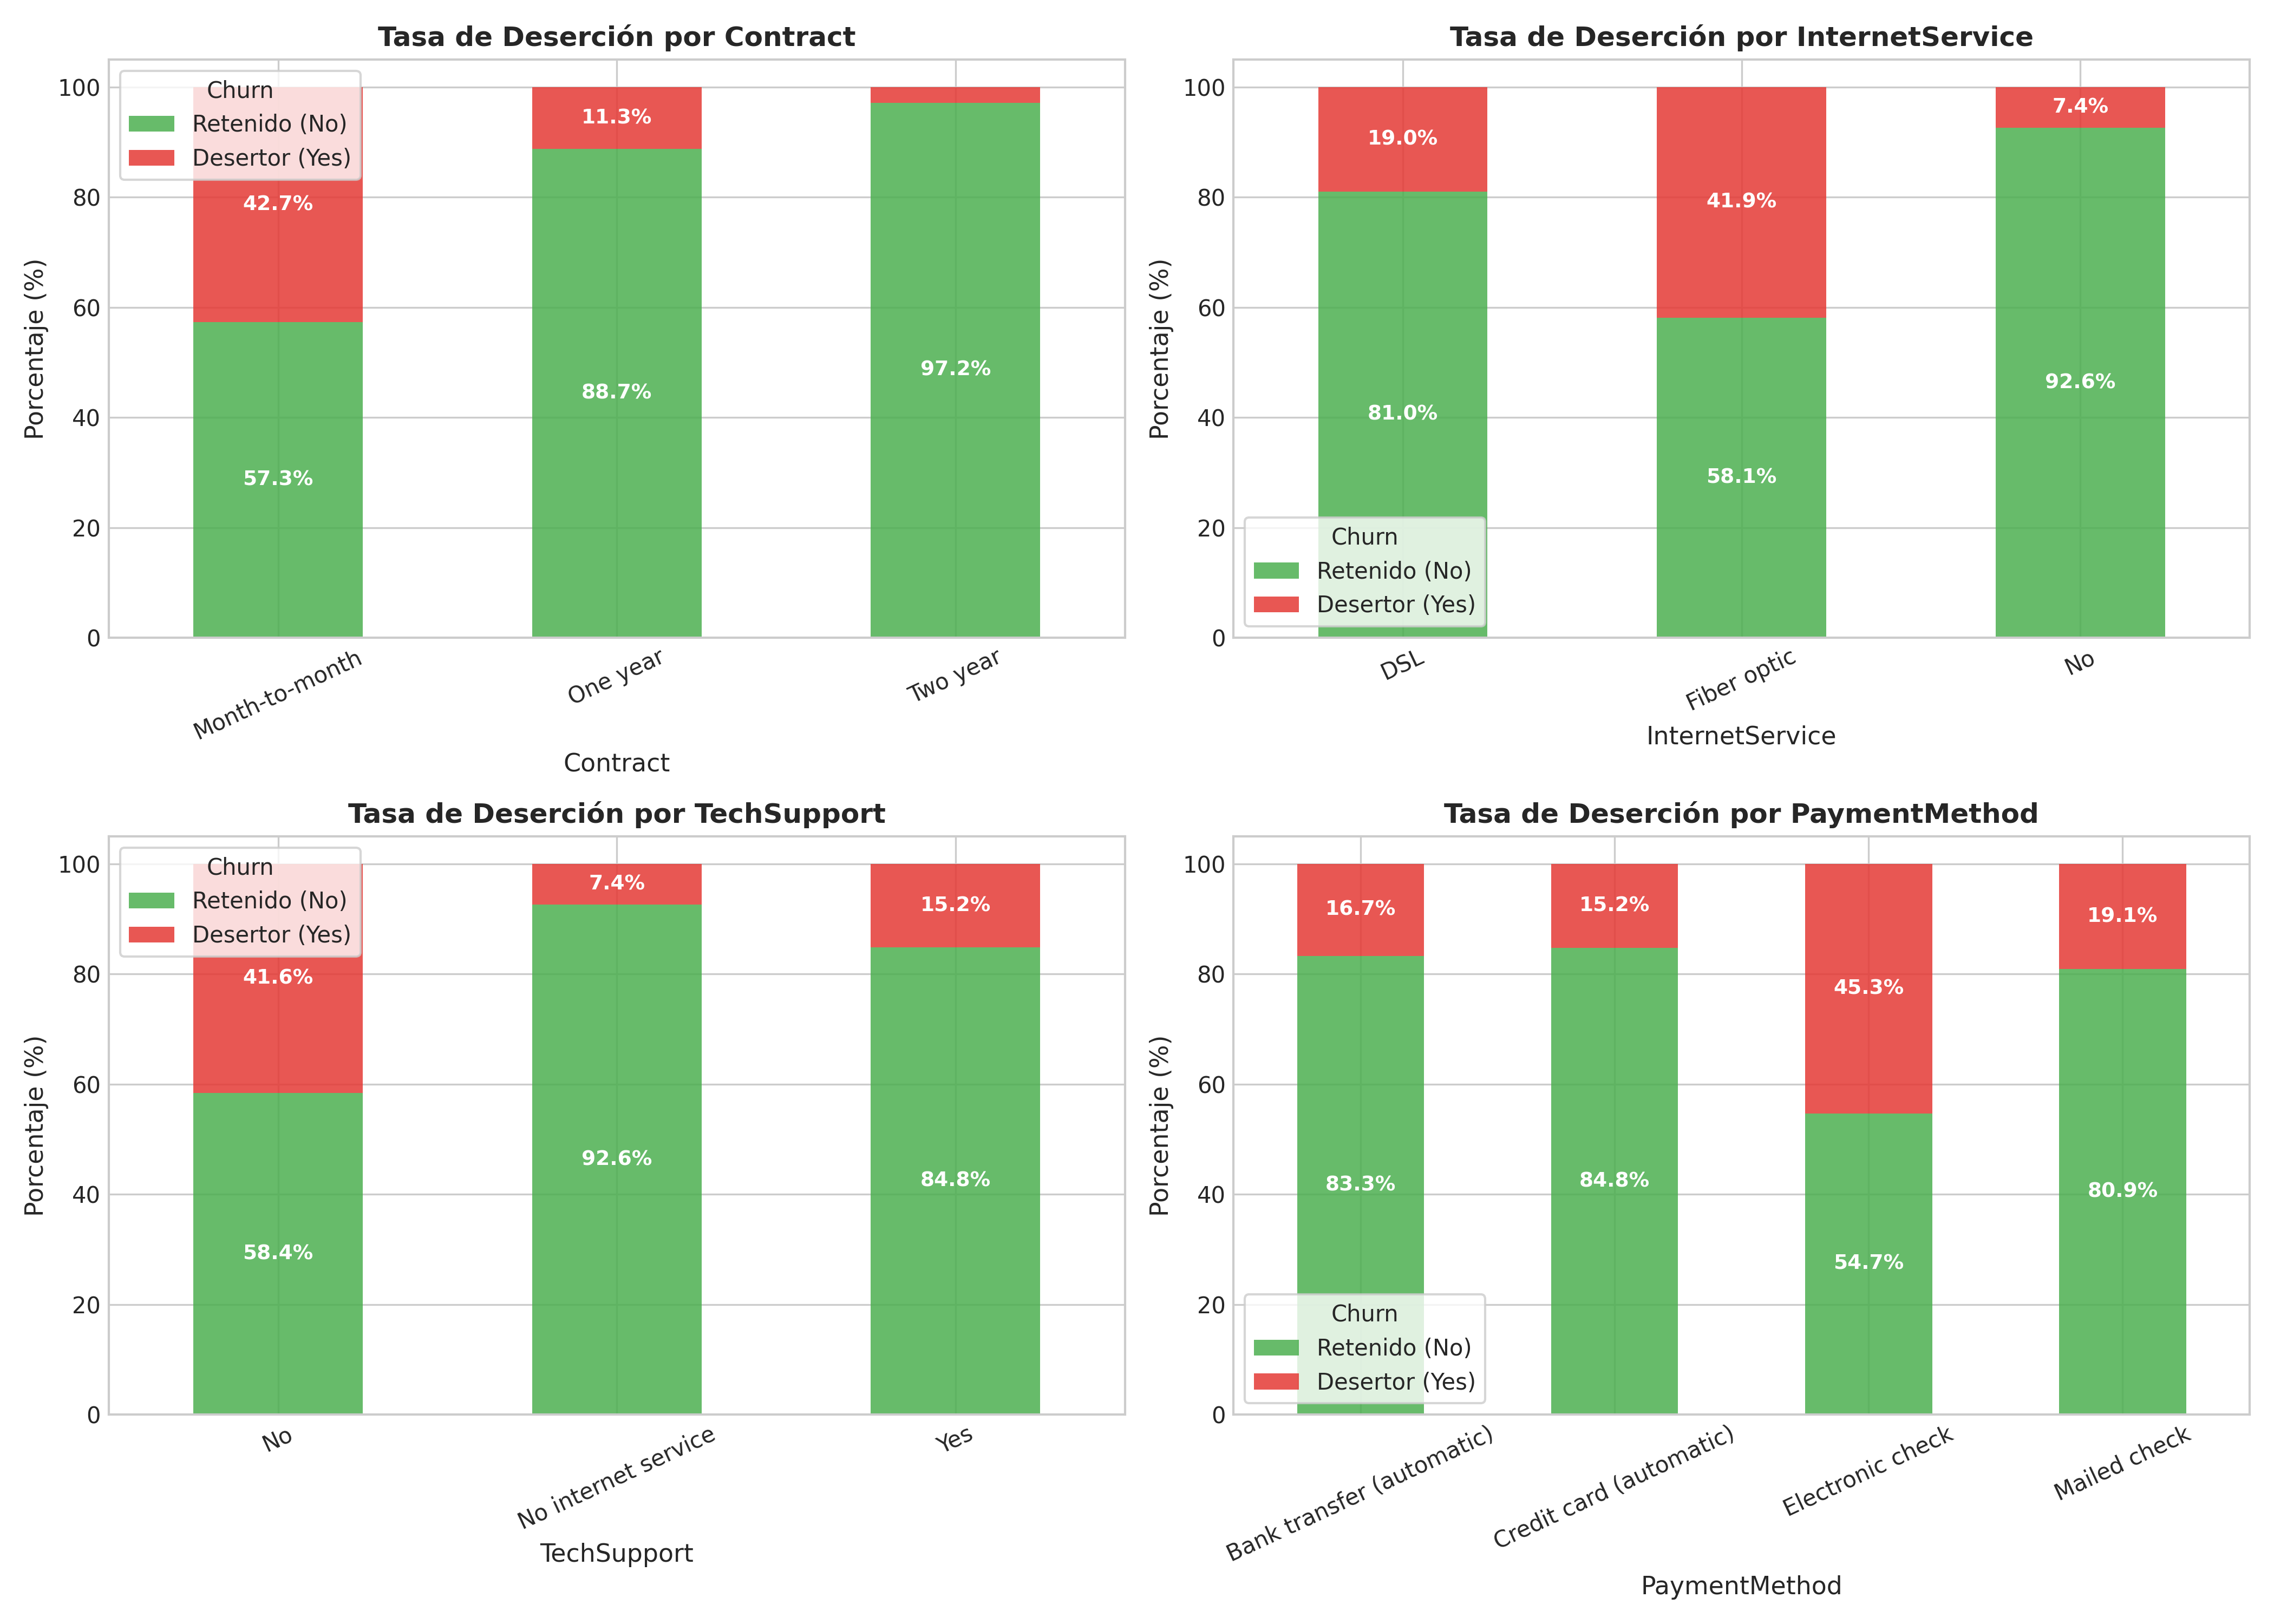
\includegraphics[width=0.95\linewidth]{figures/fig4_churn_categorical_distribution.png}
    \caption{Tasa porcentual de deserción segmentada por factores determinantes de negocio.}
    \label{fig:churn_segmentado}
\end{figure}

\subsection{Interpretación y Síntesis Analítica}
\begin{enumerate}
    \item \textbf{Impacto Decisivo de la Modalidad Contractual:} \texttt{Contract} es la variable con mayor poder explicativo del abandono ($V = 0.4101$, $p \approx 0$). Los suscriptores con contratos mes a mes (\textit{Month-to-month}) presentan una deserción del $42.7\%$, mientras que en contratos a un año y dos años la deserción se desploma a $11.3\%$ y $2.8\%$ respectivamente (Figura \ref{fig:churn_segmentado}).
    \item \textbf{Efecto Protector de los Servicios de Valor Agregado:} Las características \texttt{OnlineSecurity} ($V = 0.3474$) y \texttt{TechSupport} ($V = 0.3429$) actúan como amortiguadores de fuga. Los clientes que carecen de soporte técnico exhiben un $41.6\%$ de deserción, frente a solo un $15.2\%$ en aquellos con soporte activo.
    \item \textbf{Tecnología de Internet y Facturación:} Los usuarios con \texttt{Fiber optic} muestran una tasa de fuga del $41.9\%$, en contraste con el $19.0\%$ de usuarios con conexión \texttt{DSL}. Esto sugiere una insatisfacción latente en la relación costo/beneficio de la fibra. Paralelamente, el método de pago mediante cheque electrónico (\textit{Electronic check}) concentra una deserción del $45.3\%$.
    \item \textbf{Variables No Predictivas e Invariantes:} Se determinó rigurosamente que el género (\texttt{gender}, $p = 0.4866$) y la tenencia de telefonía fija básica (\texttt{PhoneService}, $p = 0.3388$) son estadísticamente independientes de la deserción. Este hallazgo permitirá suprimir estas columnas o descartarlas en el proceso de selección de características de la Fase 2, reduciendo la dimensionalidad sin pérdida de capacidad explicativa.
\end{enumerate}

% ==============================================================================
% SECCIÓN 4: CONCLUSIONES Y PLAN DE TRANSICIÓN A FASE 2
% ==============================================================================
\section{Conclusiones Metodológicas y Plan de Acción para la Fase 2}

\begin{enumerate}
    \item \textbf{Manejo de Calidad de Datos para Fase 2:} Se formalizó que la ausencia de los 11 valores en \texttt{TotalCharges} corresponde al mecanismo MAR condicionado por \texttt{tenure = 0}. Se realizará una imputación exacta por cero (\texttt{TotalCharges = 0.0}), garantizando la preservación completa de la muestra sin introducir distorsiones estadísticas.
    \item \textbf{Diseño de Ingeniería de Variables (Feature Engineering):} En cumplimiento estricto con los requerimientos de la Fase 2, se derivarán al menos dos variables fundamentadas en el dominio:
    \begin{itemize}
        \item \textbf{Variable Derivada 1 (\texttt{ChargeRatio}):} Razón de cobro promedio mensual $\frac{\texttt{TotalCharges}}{\texttt{tenure} + 1}$, contrastada frente a \texttt{MonthlyCharges} para detectar incrementos tarifarios recientes.
        \item \textbf{Variable Derivada 2 (\texttt{TotalServices}):} Conteo acumulado de servicios contratados ($0$ a $6$) entre seguridad, copias, soporte, póliza de dispositivo y streaming, para medir la adherencia tecnológica.
    \end{itemize}
    \item \textbf{Estrategia de Partición y Prevención de Fuga de Información (\textit{Data Leakage}):} Se dividirá el conjunto en $70\%$ Entrenamiento, $15\%$ Validación y $15\%$ Prueba mediante muestreo estratificado (\texttt{StratifiedShuffleSplit}). Toda transformación, escalado (\texttt{StandardScaler} / \texttt{RobustScaler}) y codificación (\texttt{OneHotEncoder} para nominales y \texttt{OrdinalEncoder} para contratos) se ajustará exclusivamente sobre el conjunto de entrenamiento.
    \item \textbf{Establecimiento del Modelo Base (\textit{Baseline}):} En regresión se construirá una regresión lineal univariable \texttt{TotalCharges} $\sim$ \texttt{tenure}, y en clasificación un clasificador mayoritario (\textit{DummyClassifier}) y una regresión logística simple para definir el umbral inferior de rendimiento.
\end{enumerate}

\vspace{0.8cm}
\begin{center}
    \rule{0.6\linewidth}{0.6pt}\\
    \small \textbf{Fin del Informe Técnico de la Fase 1}
\end{center}

\end{document}
